\section{Sequence diagrams}
\label{Sequence diagrams}

\todo[inline]{Premier jet, à relire et modifier !}
In this section, we will present two sequence diagrams which depict the
function of two main requirements : the creation of the groups and the creation
of the tournament table. \newline

The first diagram describe the poule creation process as we implemented it. As
you can see much of the works is automatically done by the server and the staff
only needs to check the data and make change according to his eventual
discontent, which explain why most of our diagram concern optional functions.
\newline

The second diagram describe the knock-off tournament creation process as we
implemented it on our website. \newline

\begin{figure}[!ht]
	\centering
	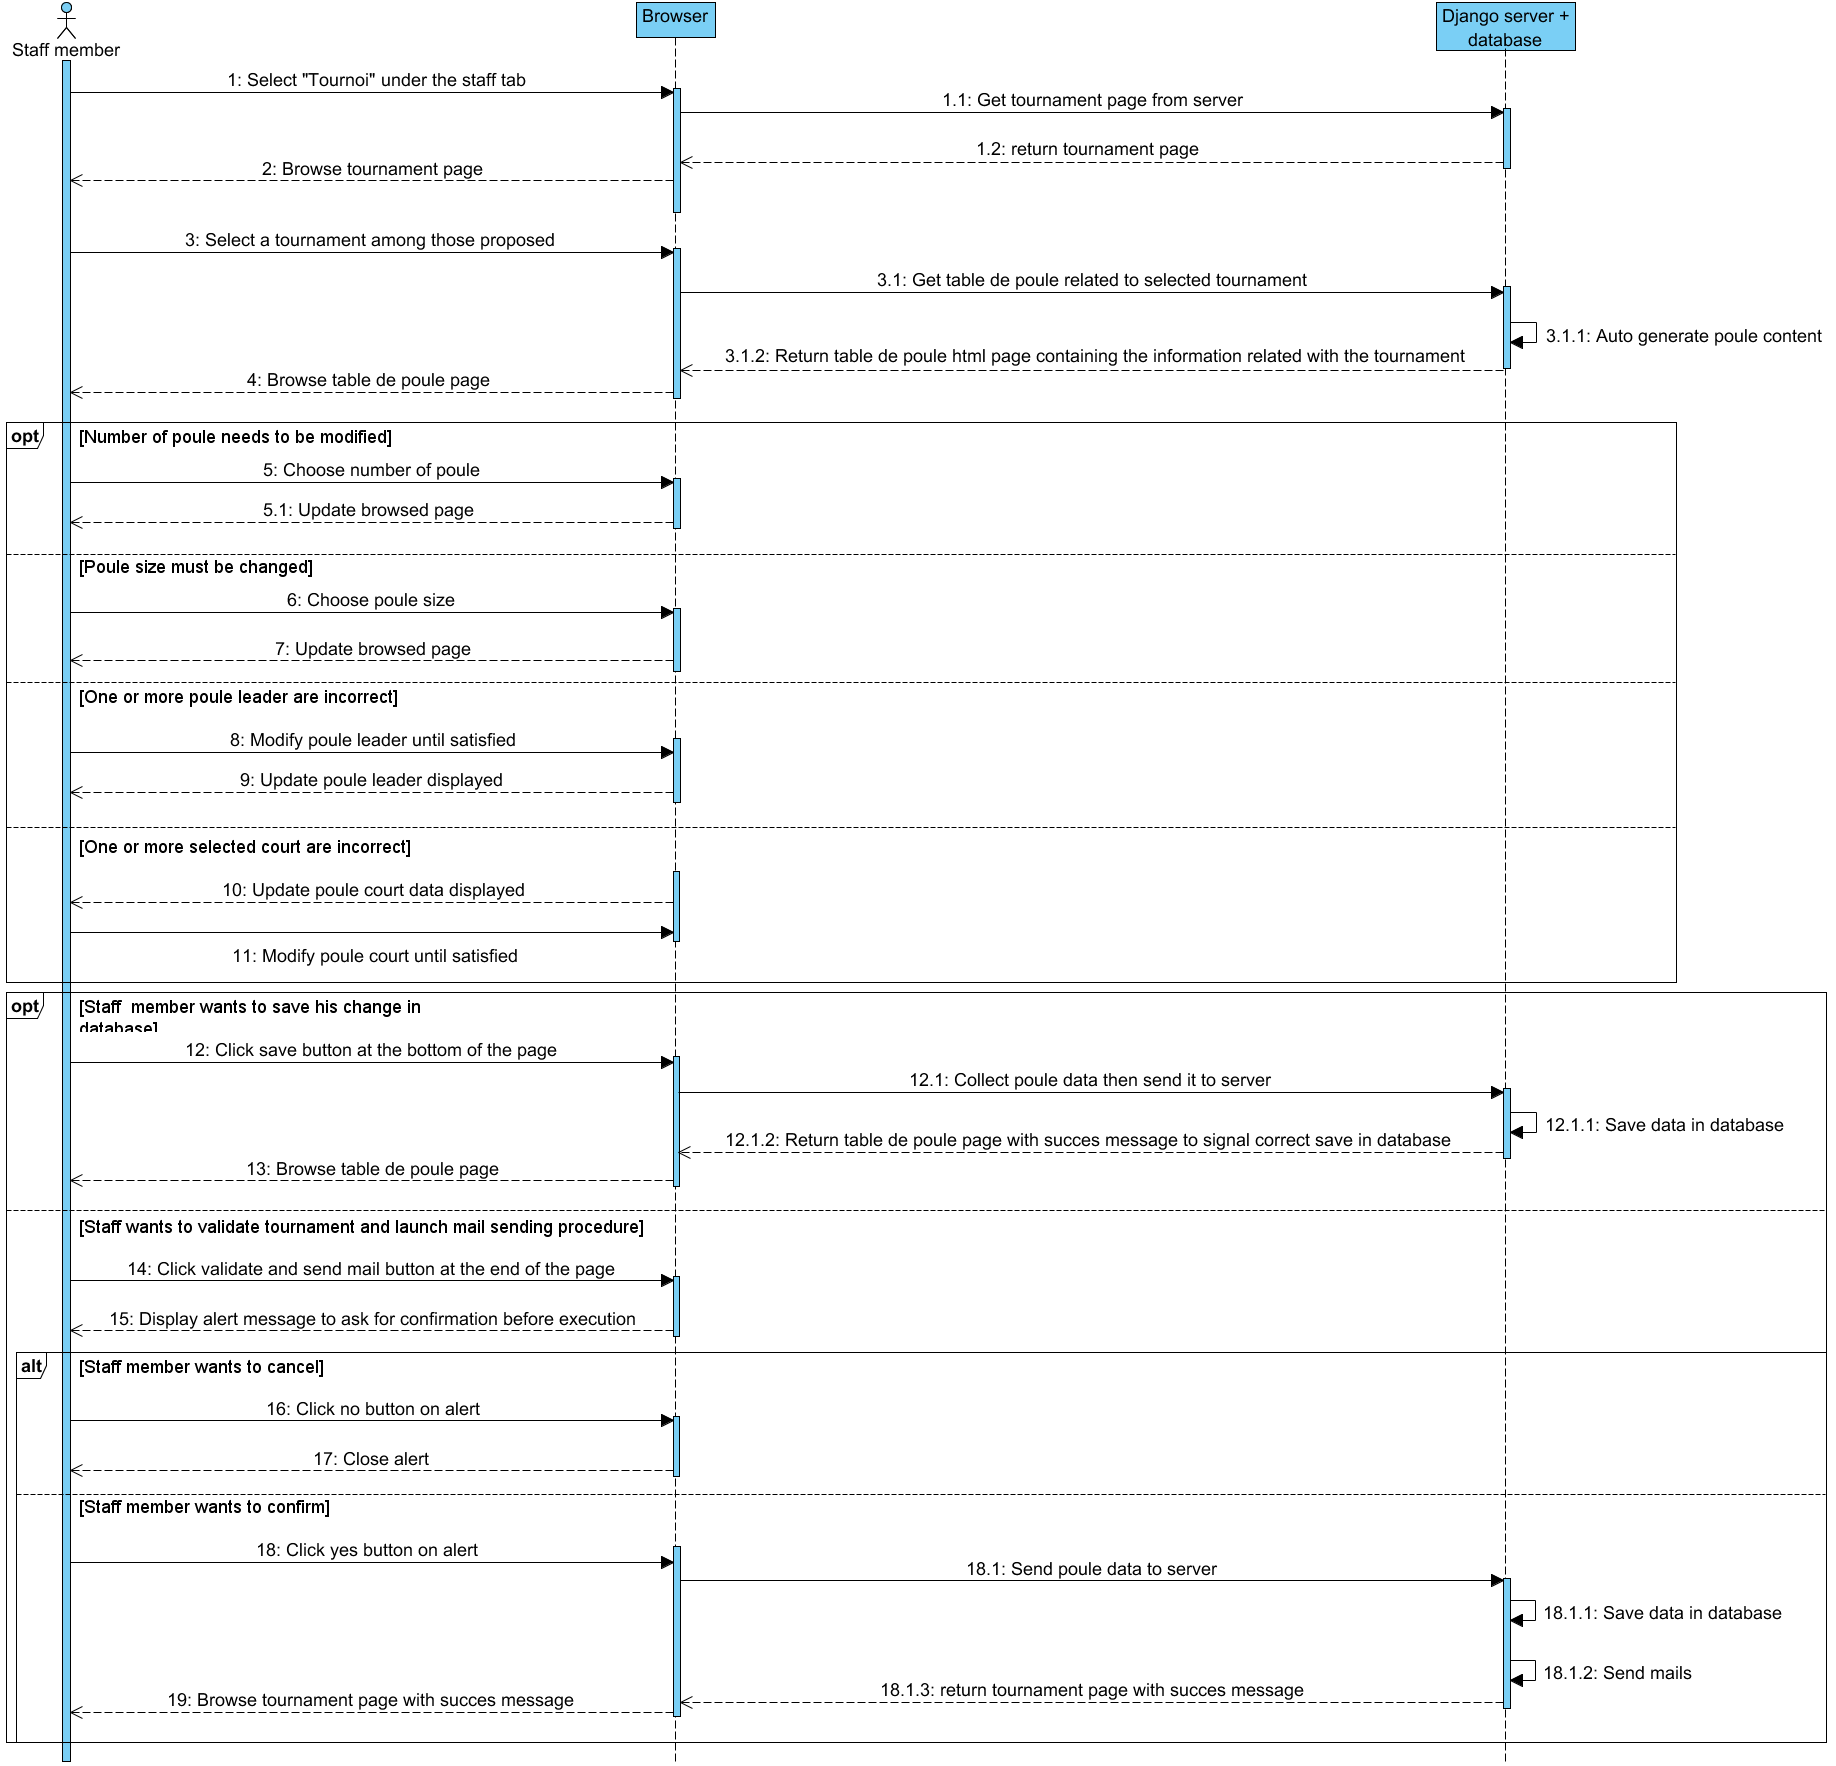
\includegraphics[width=1.1\linewidth]{poule.png}
	\caption{Sequence diagram of the poule creation process}
	\label{fig:length_eight_mouse}
\end{figure}
\FloatBarrier

\begin{figure}[!ht]
	\centering
	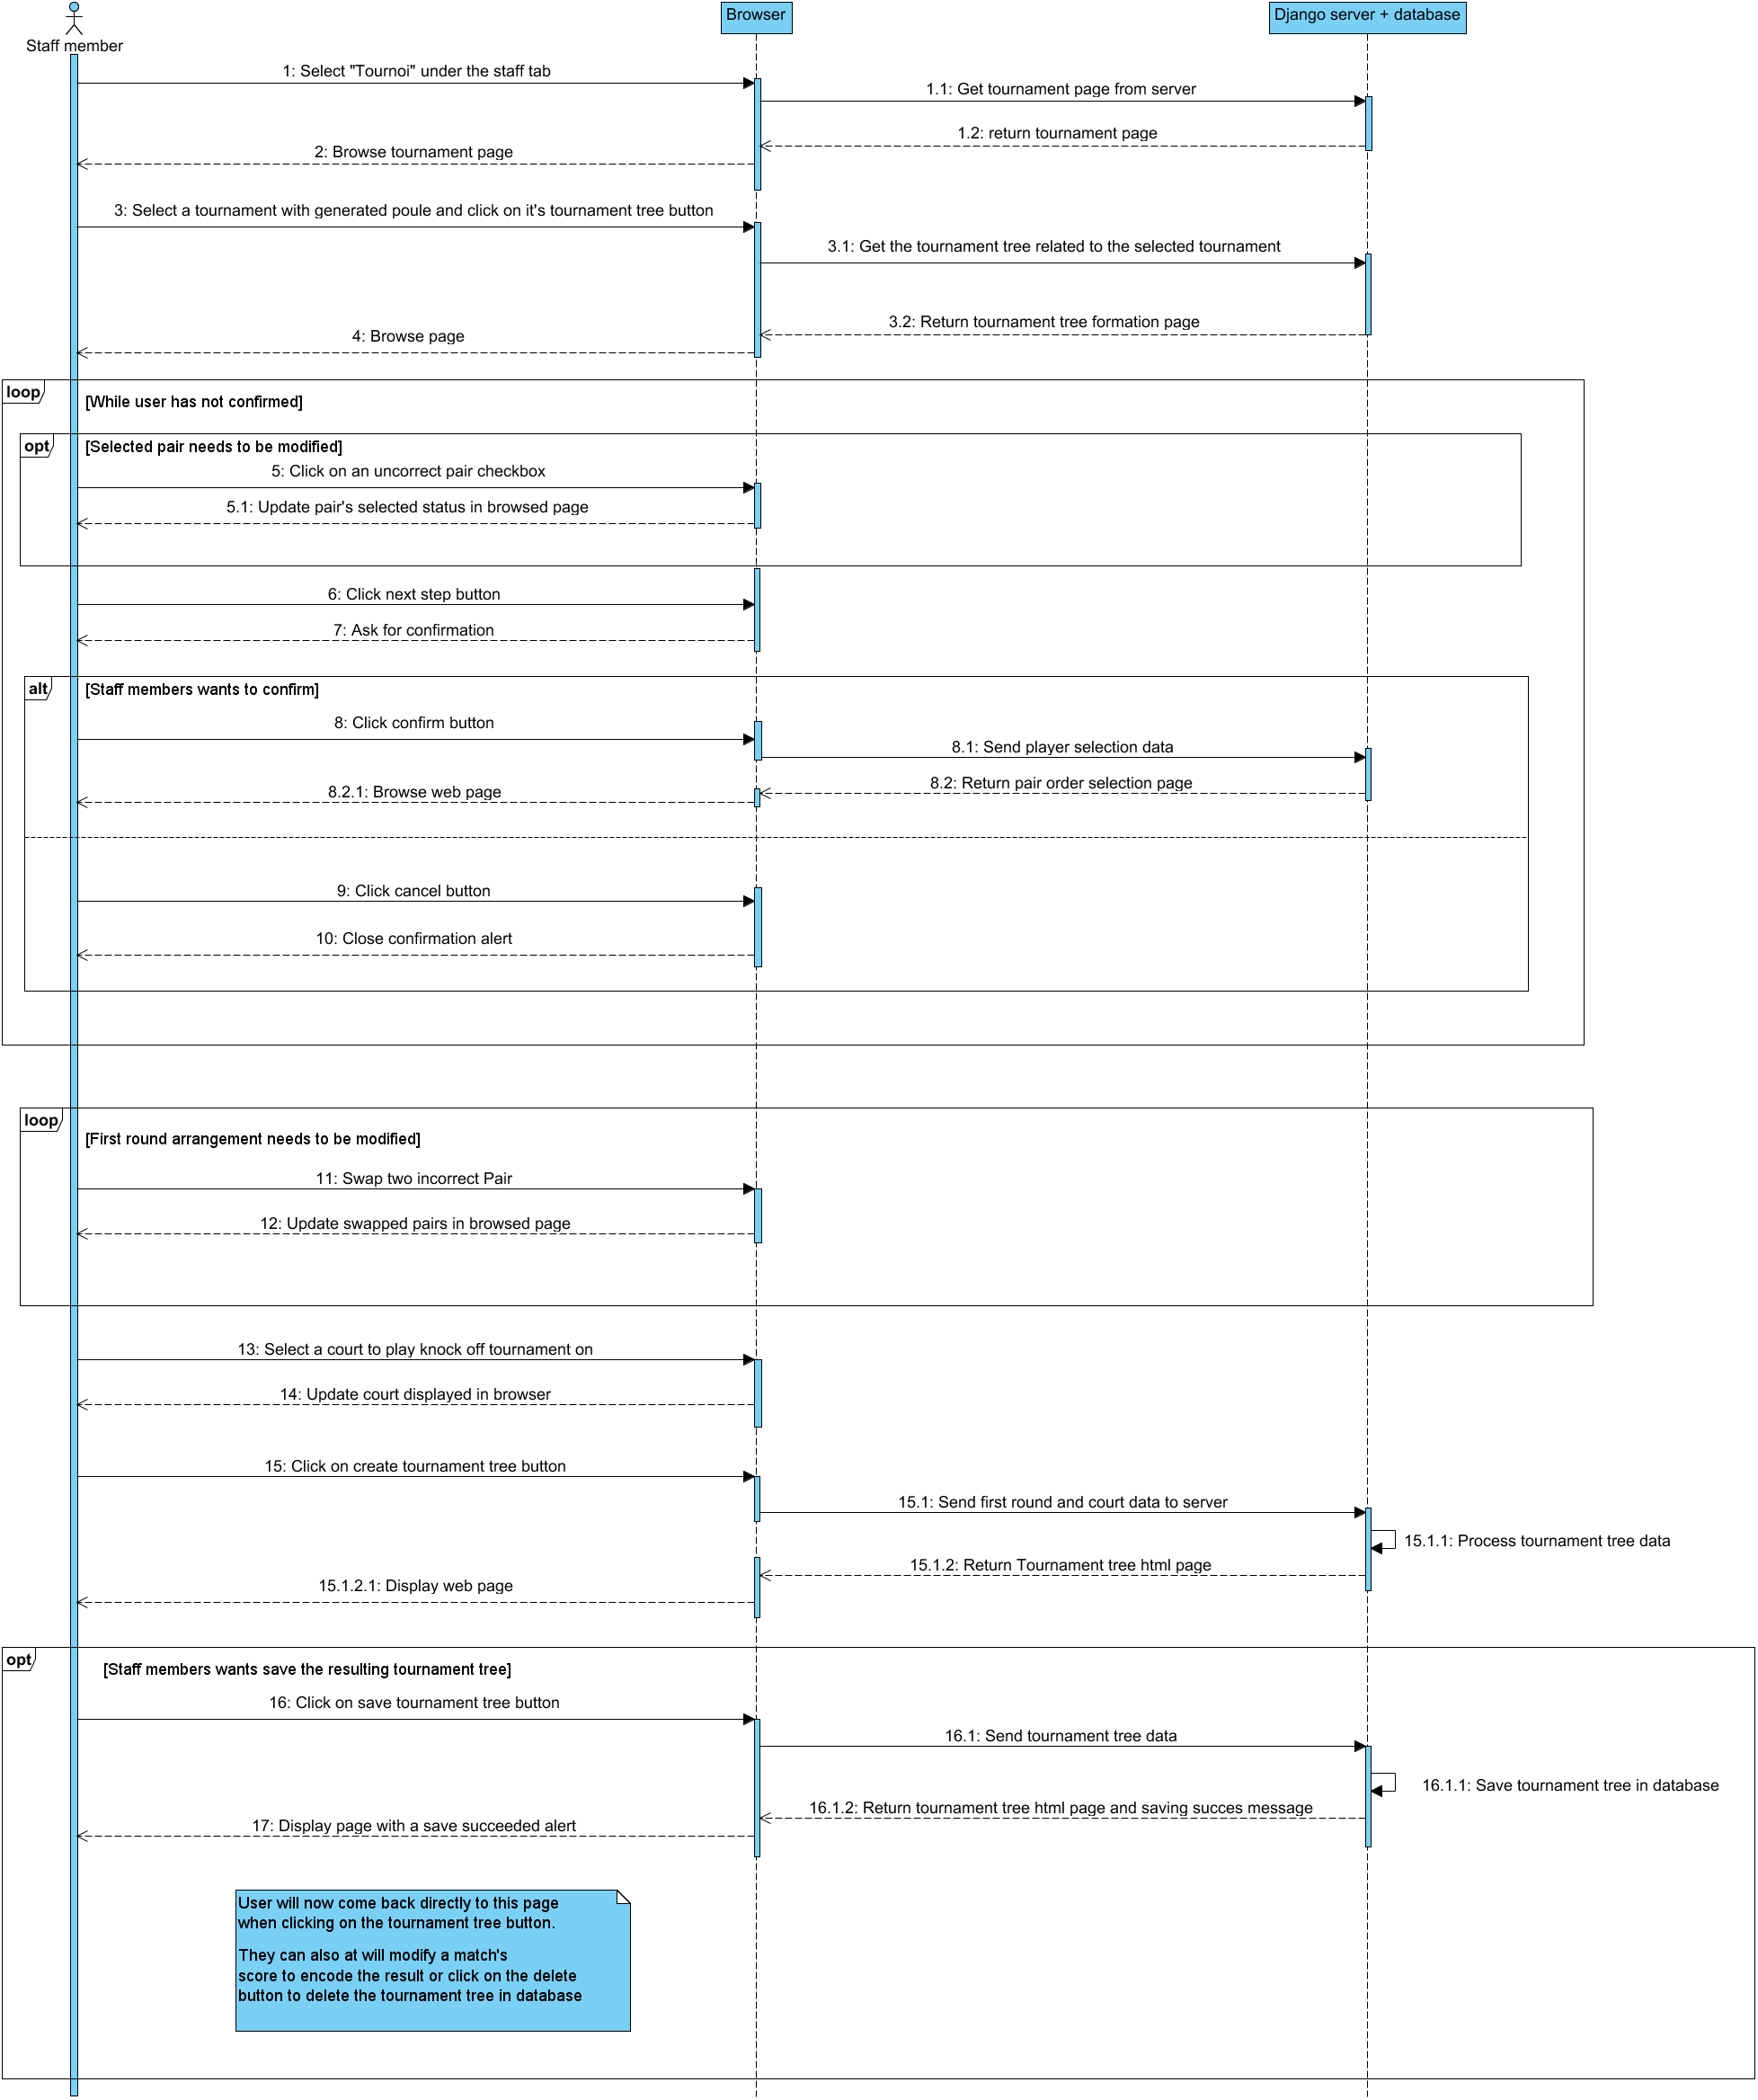
\includegraphics[width=1.1\linewidth]{tournament.png}
	\caption{Sequence diagram of the knock-off tournament creation process}
	\label{fig:length_eight_mouse}
\end{figure}
\FloatBarrier
